\documentclass[]{article}
\usepackage{lmodern}
\usepackage{amssymb,amsmath}
\usepackage{ifxetex,ifluatex}
\usepackage{fixltx2e} % provides \textsubscript
\ifnum 0\ifxetex 1\fi\ifluatex 1\fi=0 % if pdftex
  \usepackage[T1]{fontenc}
  \usepackage[utf8]{inputenc}
\else % if luatex or xelatex
  \ifxetex
    \usepackage{mathspec}
  \else
    \usepackage{fontspec}
  \fi
  \defaultfontfeatures{Ligatures=TeX,Scale=MatchLowercase}
\fi
% use upquote if available, for straight quotes in verbatim environments
\IfFileExists{upquote.sty}{\usepackage{upquote}}{}
% use microtype if available
\IfFileExists{microtype.sty}{%
\usepackage{microtype}
\UseMicrotypeSet[protrusion]{basicmath} % disable protrusion for tt fonts
}{}
\usepackage[margin=1in]{geometry}
\usepackage{hyperref}
\hypersetup{unicode=true,
            pdftitle={Low level of covariance simulation},
            pdfauthor={Xuelong Wang},
            pdfborder={0 0 0},
            breaklinks=true}
\urlstyle{same}  % don't use monospace font for urls
\usepackage{graphicx,grffile}
\makeatletter
\def\maxwidth{\ifdim\Gin@nat@width>\linewidth\linewidth\else\Gin@nat@width\fi}
\def\maxheight{\ifdim\Gin@nat@height>\textheight\textheight\else\Gin@nat@height\fi}
\makeatother
% Scale images if necessary, so that they will not overflow the page
% margins by default, and it is still possible to overwrite the defaults
% using explicit options in \includegraphics[width, height, ...]{}
\setkeys{Gin}{width=\maxwidth,height=\maxheight,keepaspectratio}
\IfFileExists{parskip.sty}{%
\usepackage{parskip}
}{% else
\setlength{\parindent}{0pt}
\setlength{\parskip}{6pt plus 2pt minus 1pt}
}
\setlength{\emergencystretch}{3em}  % prevent overfull lines
\providecommand{\tightlist}{%
  \setlength{\itemsep}{0pt}\setlength{\parskip}{0pt}}
\setcounter{secnumdepth}{5}
% Redefines (sub)paragraphs to behave more like sections
\ifx\paragraph\undefined\else
\let\oldparagraph\paragraph
\renewcommand{\paragraph}[1]{\oldparagraph{#1}\mbox{}}
\fi
\ifx\subparagraph\undefined\else
\let\oldsubparagraph\subparagraph
\renewcommand{\subparagraph}[1]{\oldsubparagraph{#1}\mbox{}}
\fi

%%% Use protect on footnotes to avoid problems with footnotes in titles
\let\rmarkdownfootnote\footnote%
\def\footnote{\protect\rmarkdownfootnote}

%%% Change title format to be more compact
\usepackage{titling}

% Create subtitle command for use in maketitle
\providecommand{\subtitle}[1]{
  \posttitle{
    \begin{center}\large#1\end{center}
    }
}

\setlength{\droptitle}{-2em}

  \title{Low level of covariance simulation}
    \pretitle{\vspace{\droptitle}\centering\huge}
  \posttitle{\par}
    \author{Xuelong Wang}
    \preauthor{\centering\large\emph}
  \postauthor{\par}
      \predate{\centering\large\emph}
  \postdate{\par}
    \date{2019-08-23}

\usepackage{float,amsmath, bbm, siunitx, bm}
\usepackage{pdfpages}
\floatplacement{figure}{H}
\newcommand{\indep}{\rotatebox[origin=c]{90}{$\models$}}

\begin{document}
\maketitle

{
\setcounter{tocdepth}{2}
\tableofcontents
}
\section{Motivation}\label{motivation}

Based on the investigation of the covariance matrix patter of the PCBs
from 1999 - 2004, we found some patterns that appears among the
covariance matrix of PCBs from differert years. Besides, we also use the
historical data to estimate the covariance matrix, then use the sample
covariance matrix to decorrelate the PCBs for each year. For most years,
the decorrelation procedure can reduce the correlation, e.g 1999-2001,
but there are some years which the correlations still are high after
decorrelation, e.g 2005-2006.

Since we are trying to borrow information of historical dataset, the
decorrelated data will probably not be perfert uncorrelted. In other
words, we will end up with data with low correlations among their
coveriates. So the goal of this report is to see if the GCTA and
EigenPrism method could work well under the low correlation setup.

\section{setup}\label{setup}

\subsection{Sample covariance matrix}\label{sample-covariance-matrix}

I use two different sample covariane matrices: 1999-2001 and 2007 -2008.

\begin{figure}
\centering
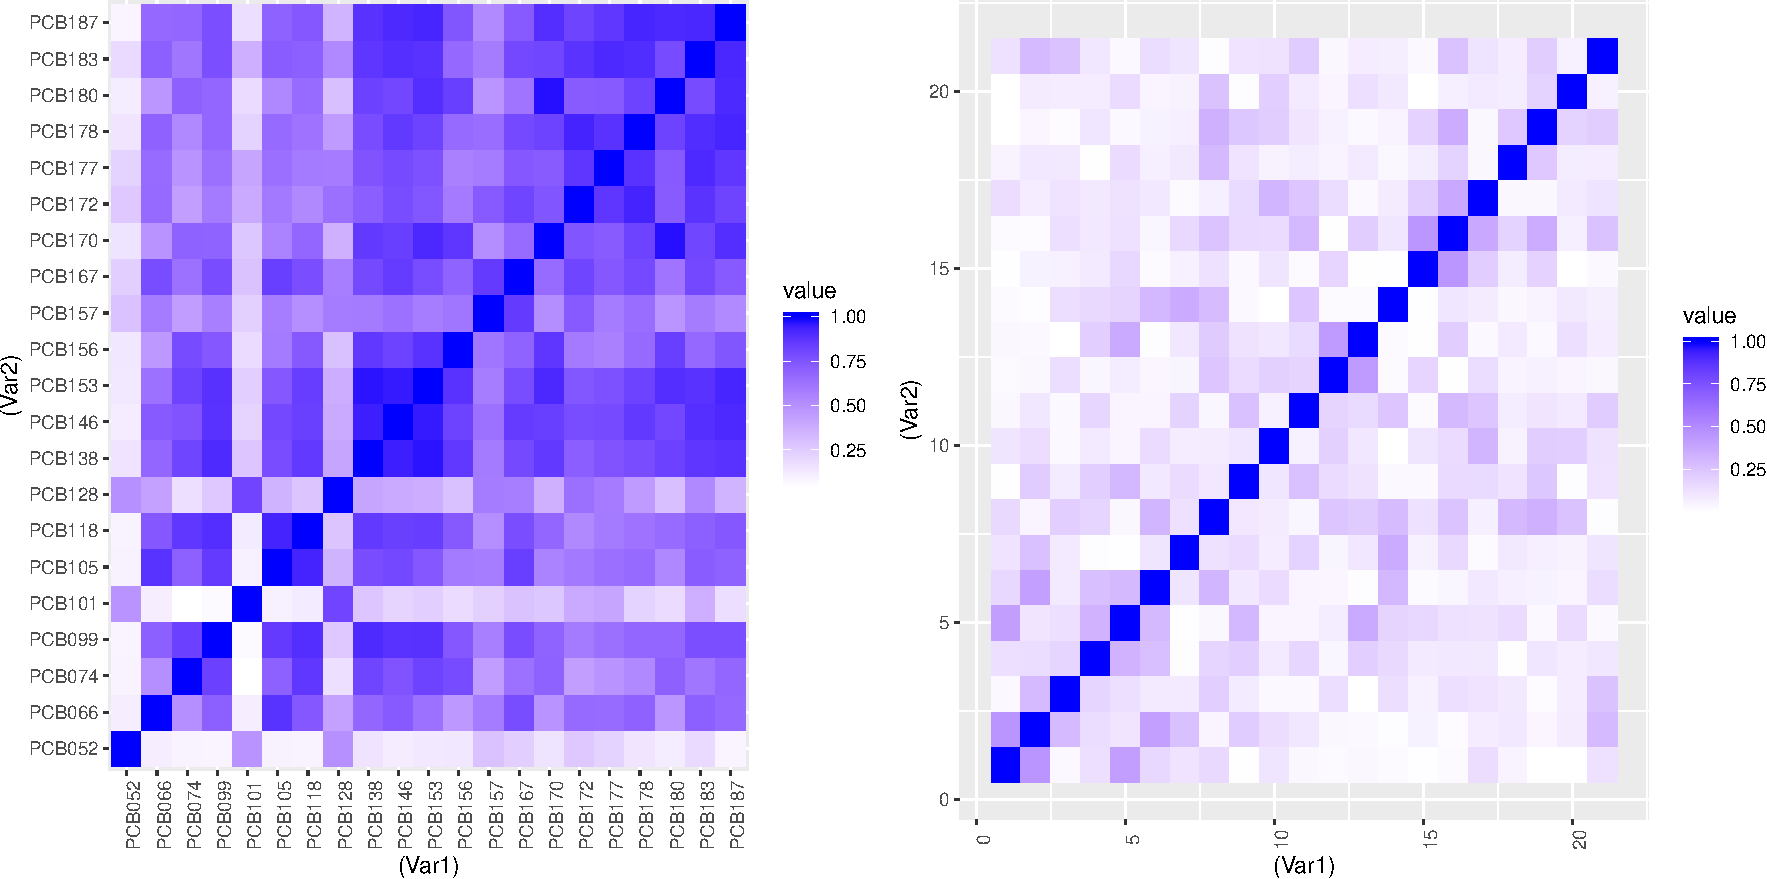
\includegraphics{Low_levels_covariance_files/figure-latex/unnamed-chunk-2-1.pdf}
\caption{1999-2000}
\end{figure}

\begin{figure}
\centering
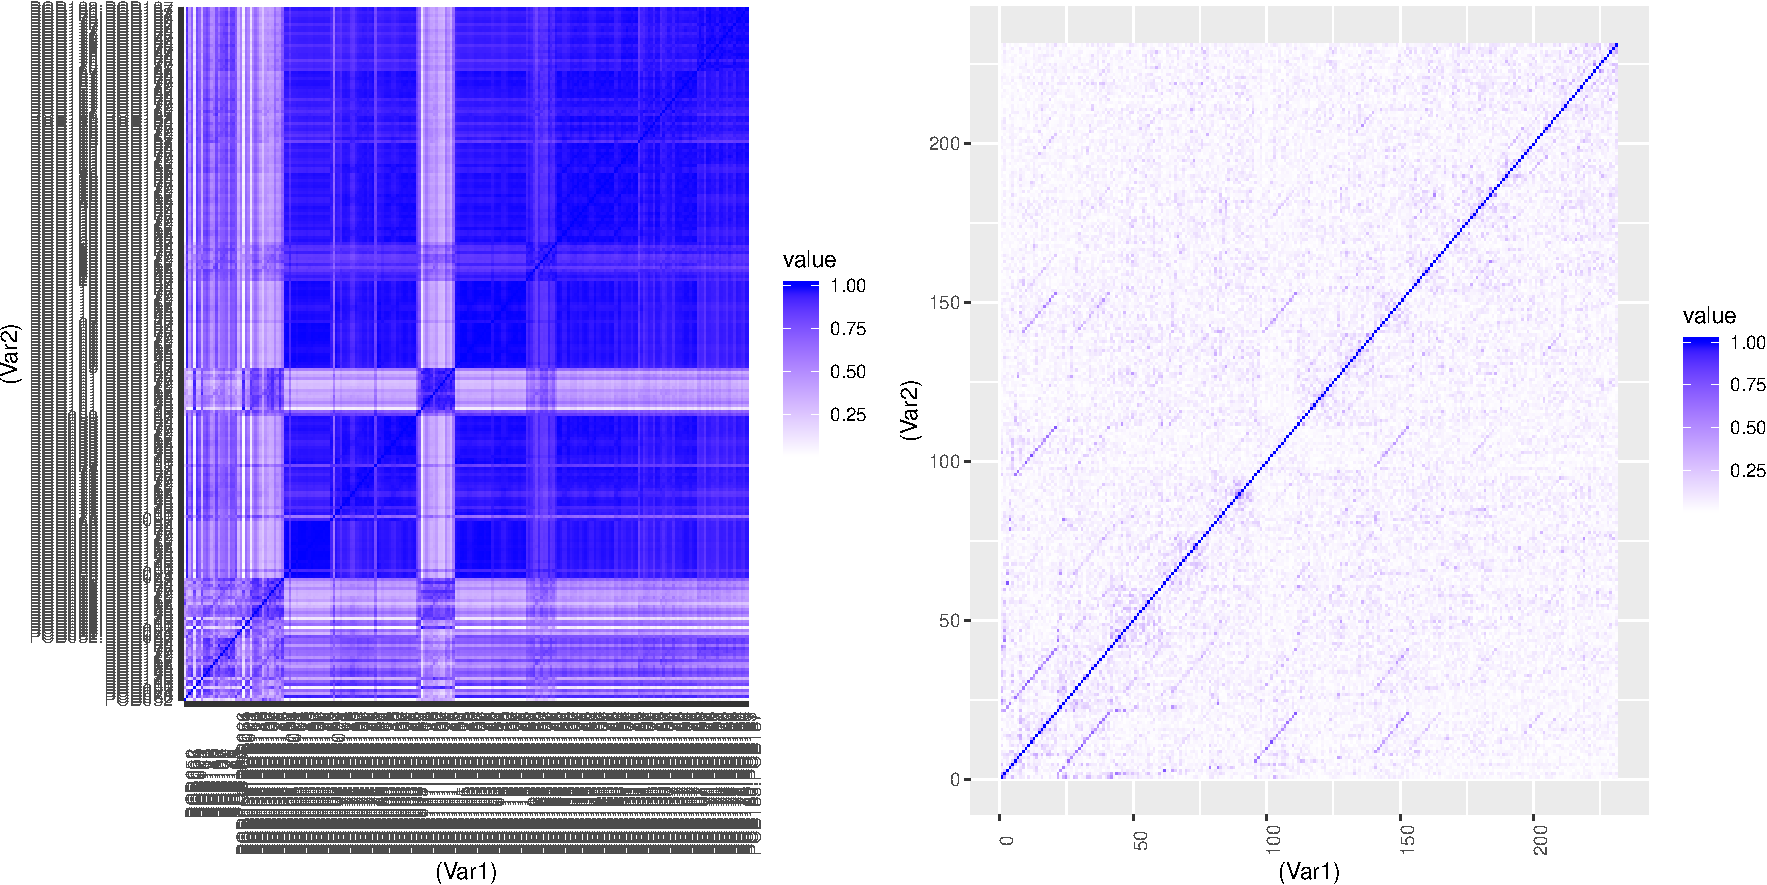
\includegraphics{Low_levels_covariance_files/figure-latex/unnamed-chunk-3-1.pdf}
\caption{Combined main and interaction 1999-2000}
\end{figure}

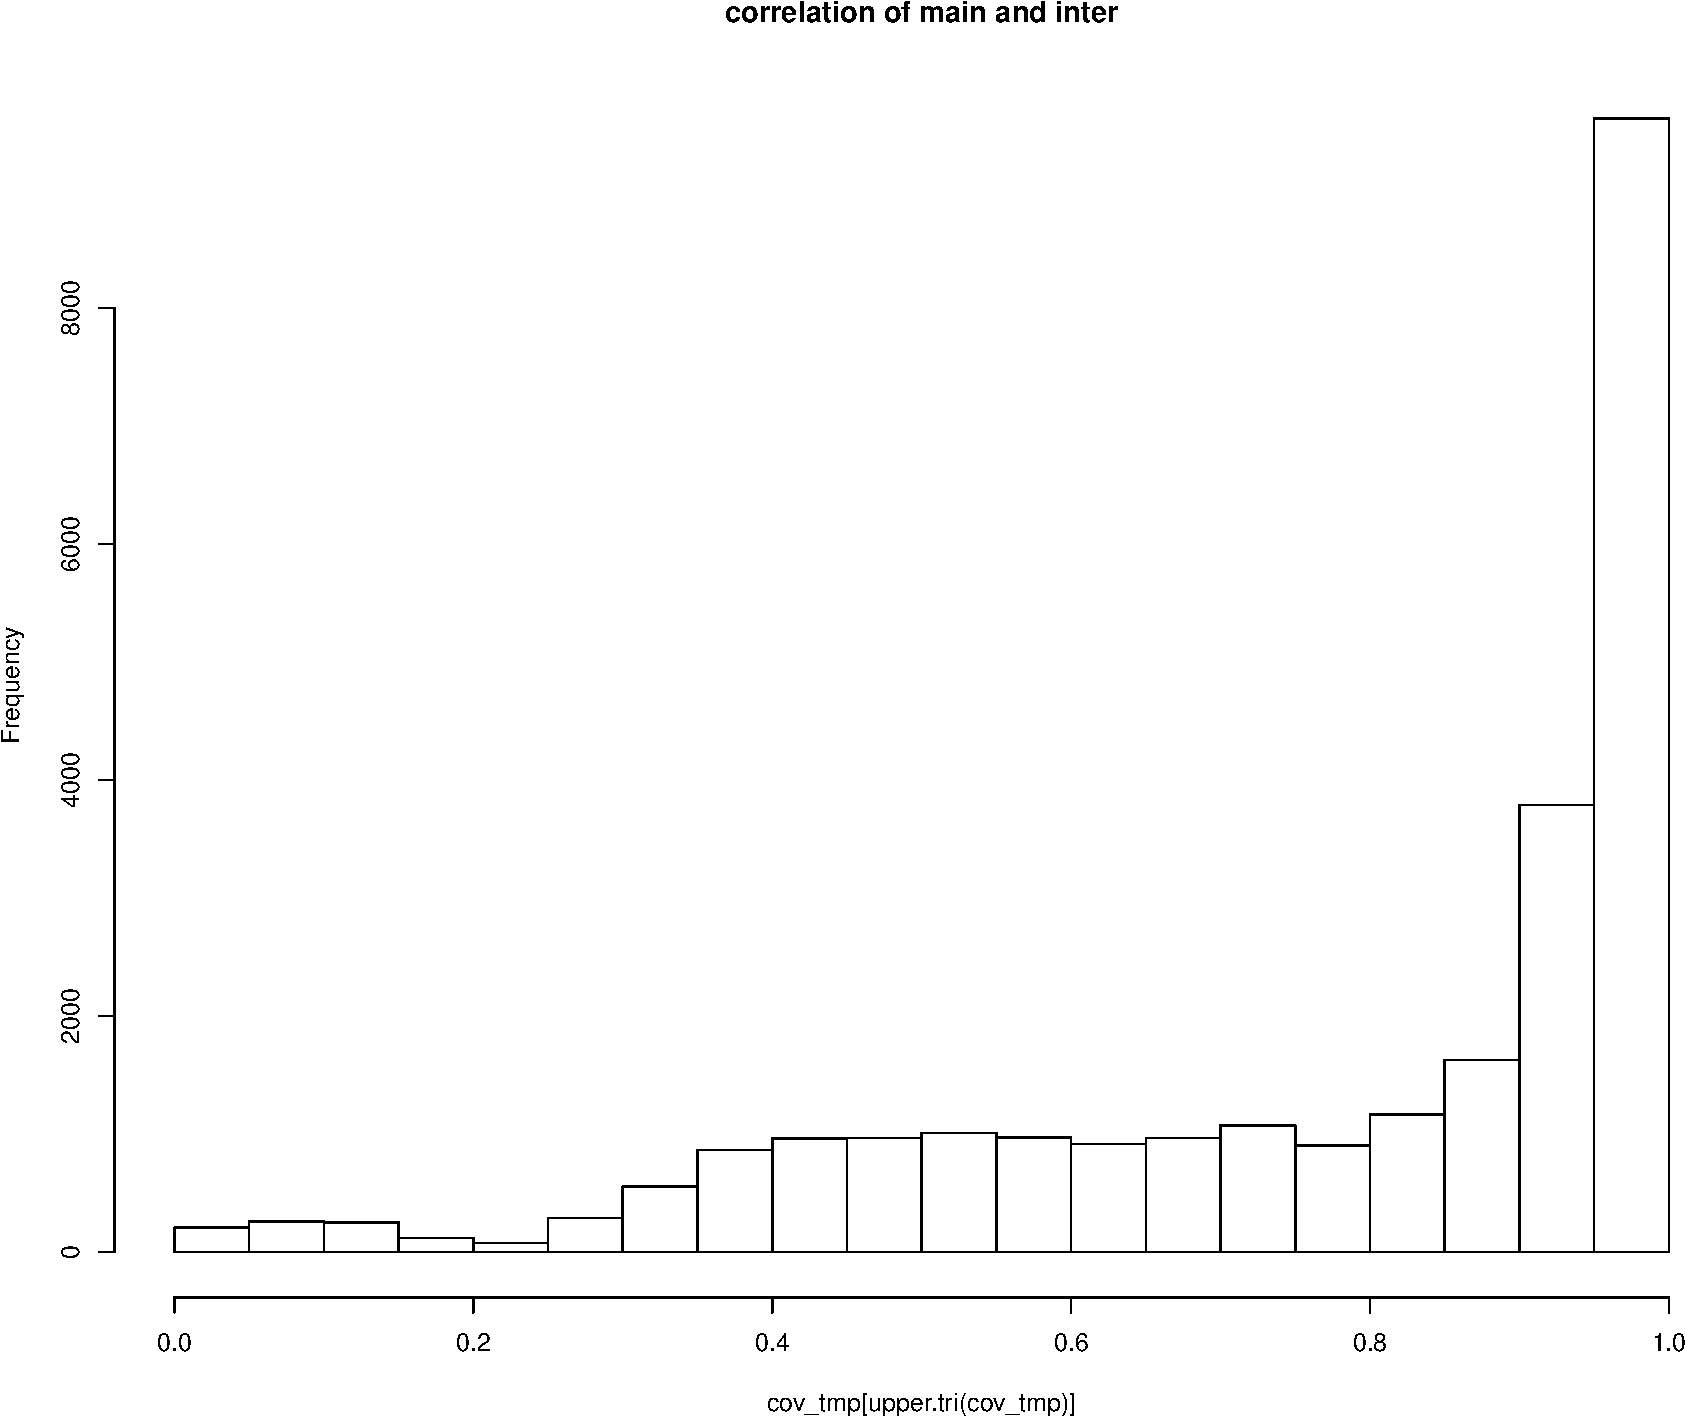
\includegraphics{Low_levels_covariance_files/figure-latex/unnamed-chunk-4-1.pdf}

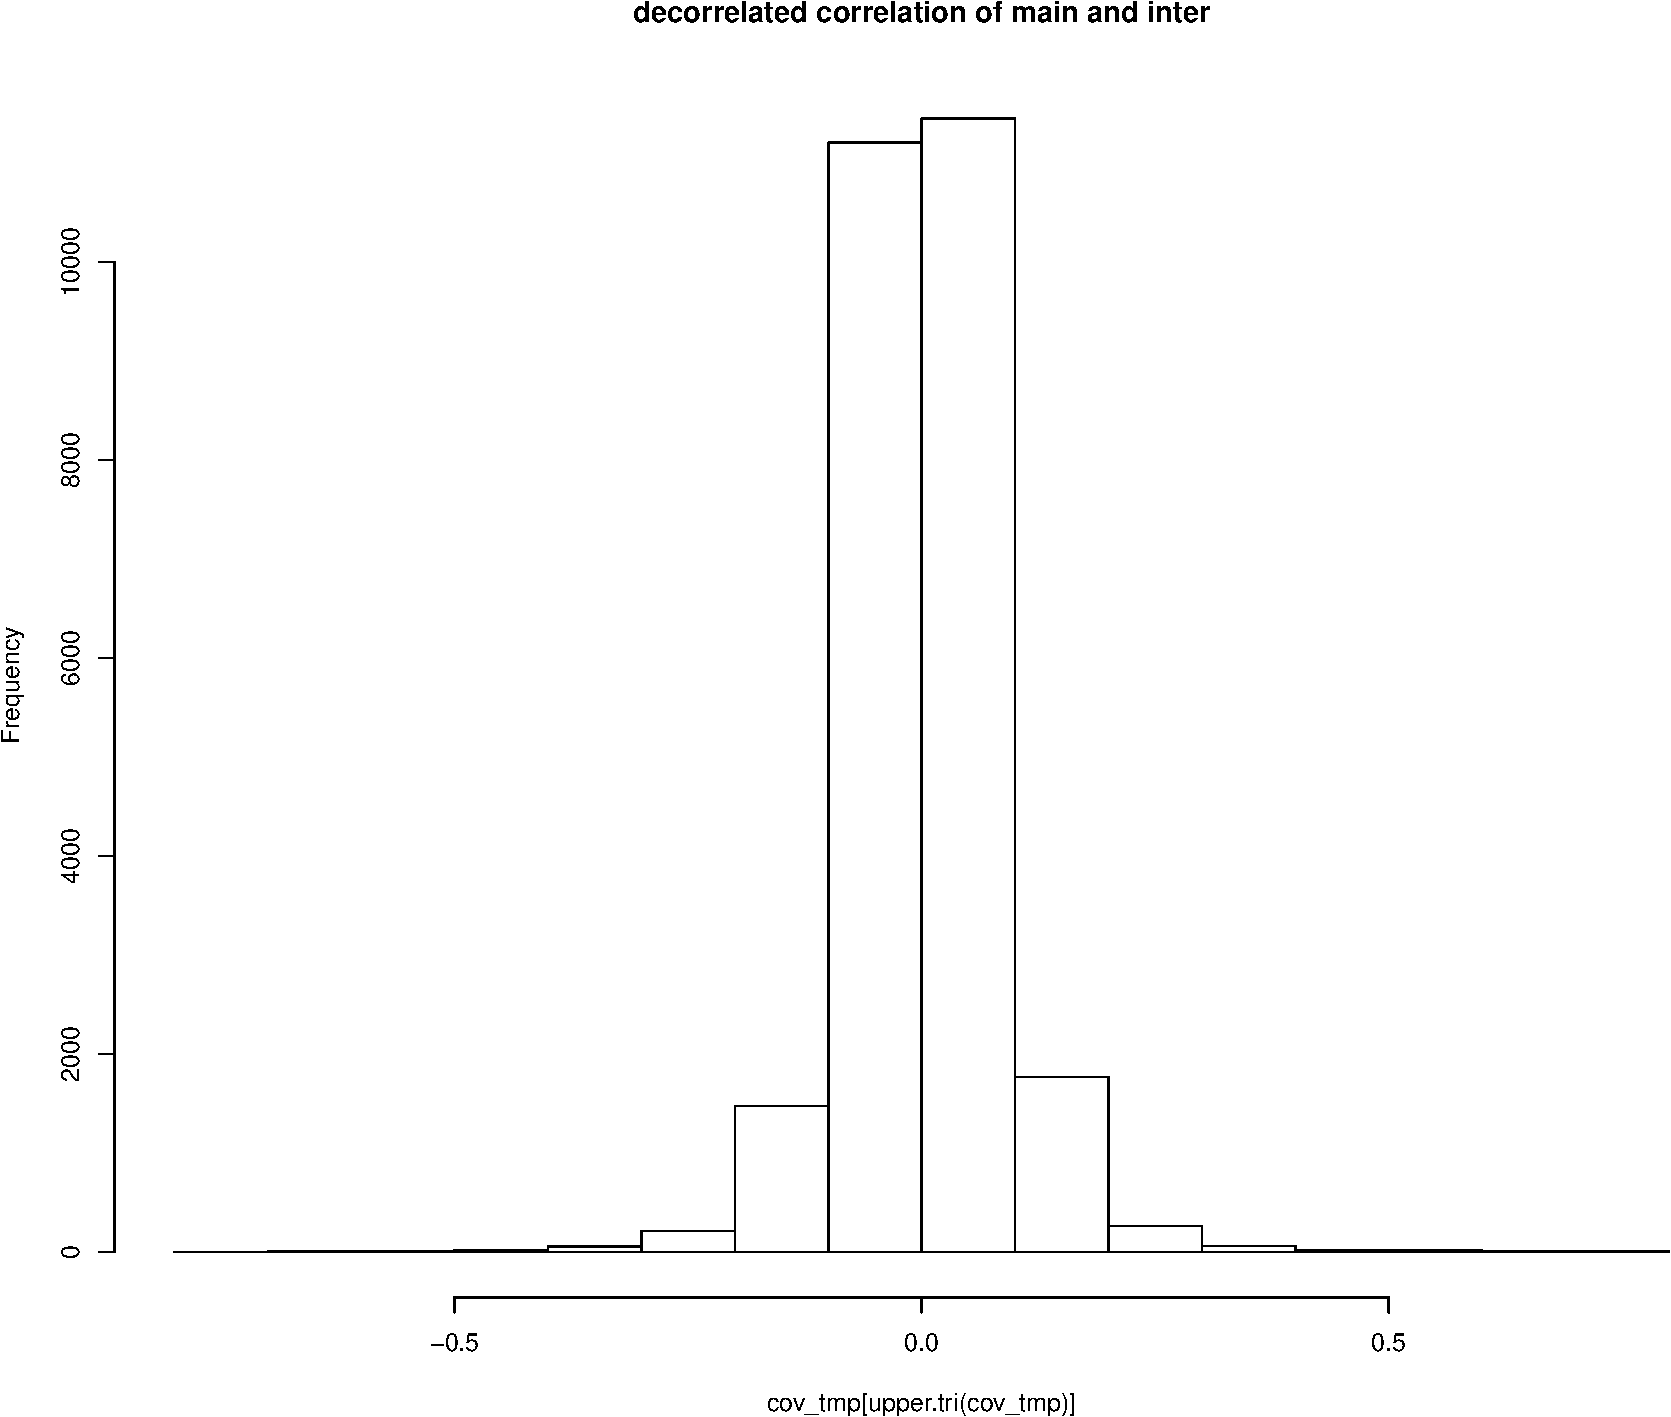
\includegraphics{Low_levels_covariance_files/figure-latex/unnamed-chunk-5-1.pdf}

\begin{figure}
\centering
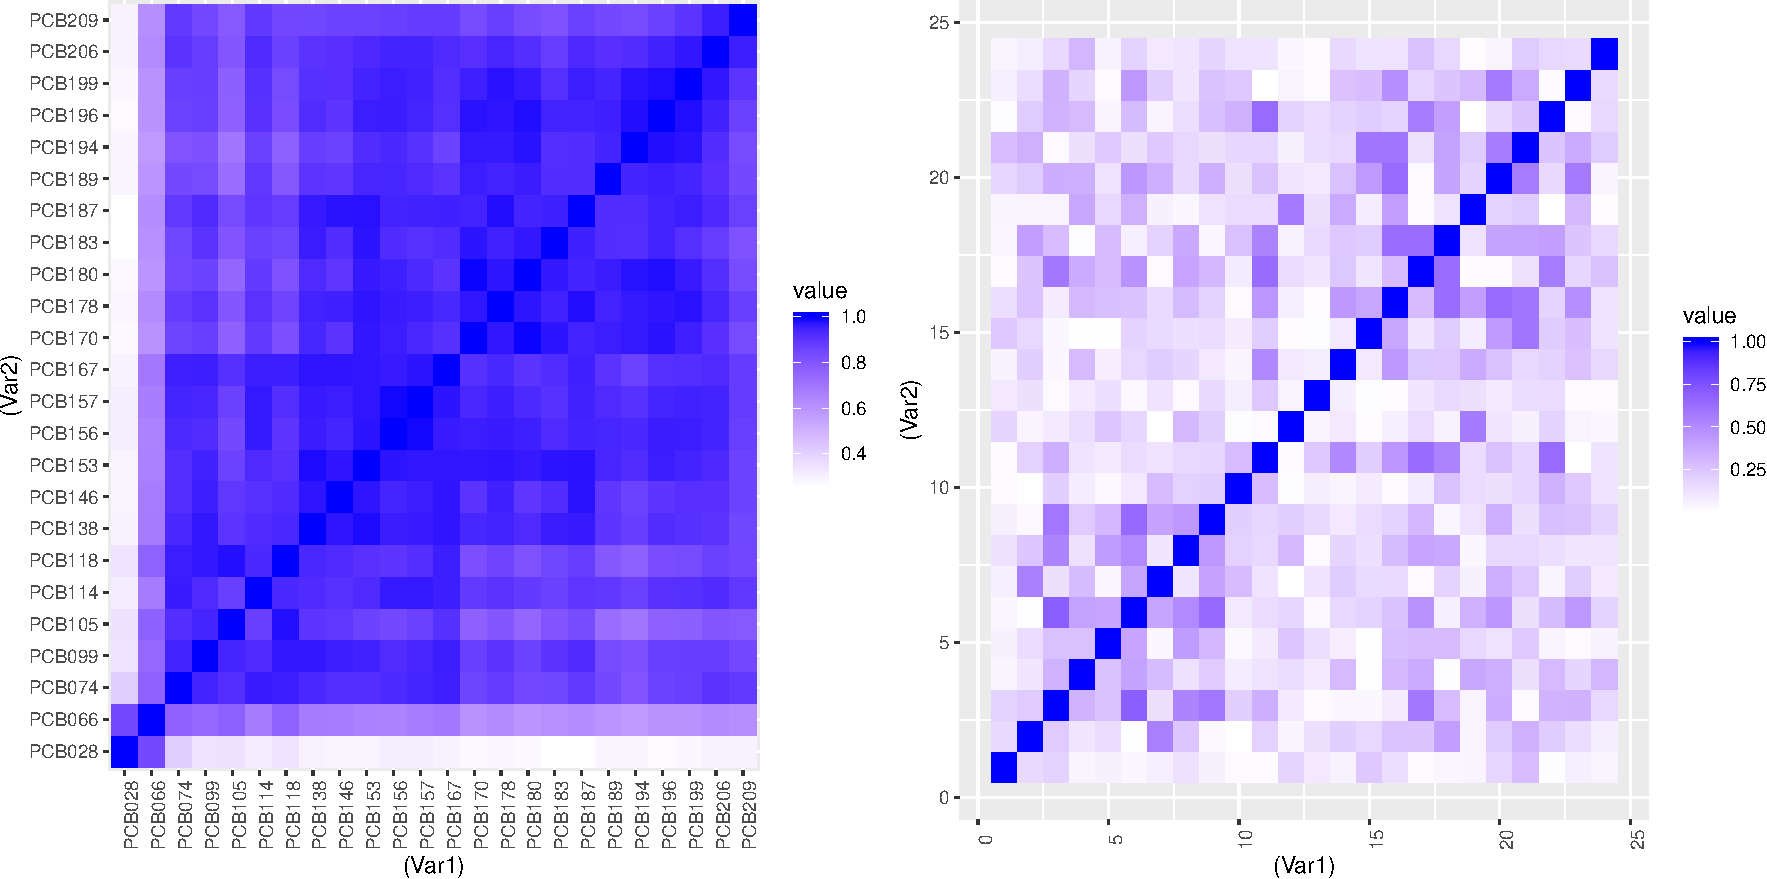
\includegraphics{Low_levels_covariance_files/figure-latex/unnamed-chunk-7-1.pdf}
\caption{2005-2006}
\end{figure}

\begin{figure}
\centering
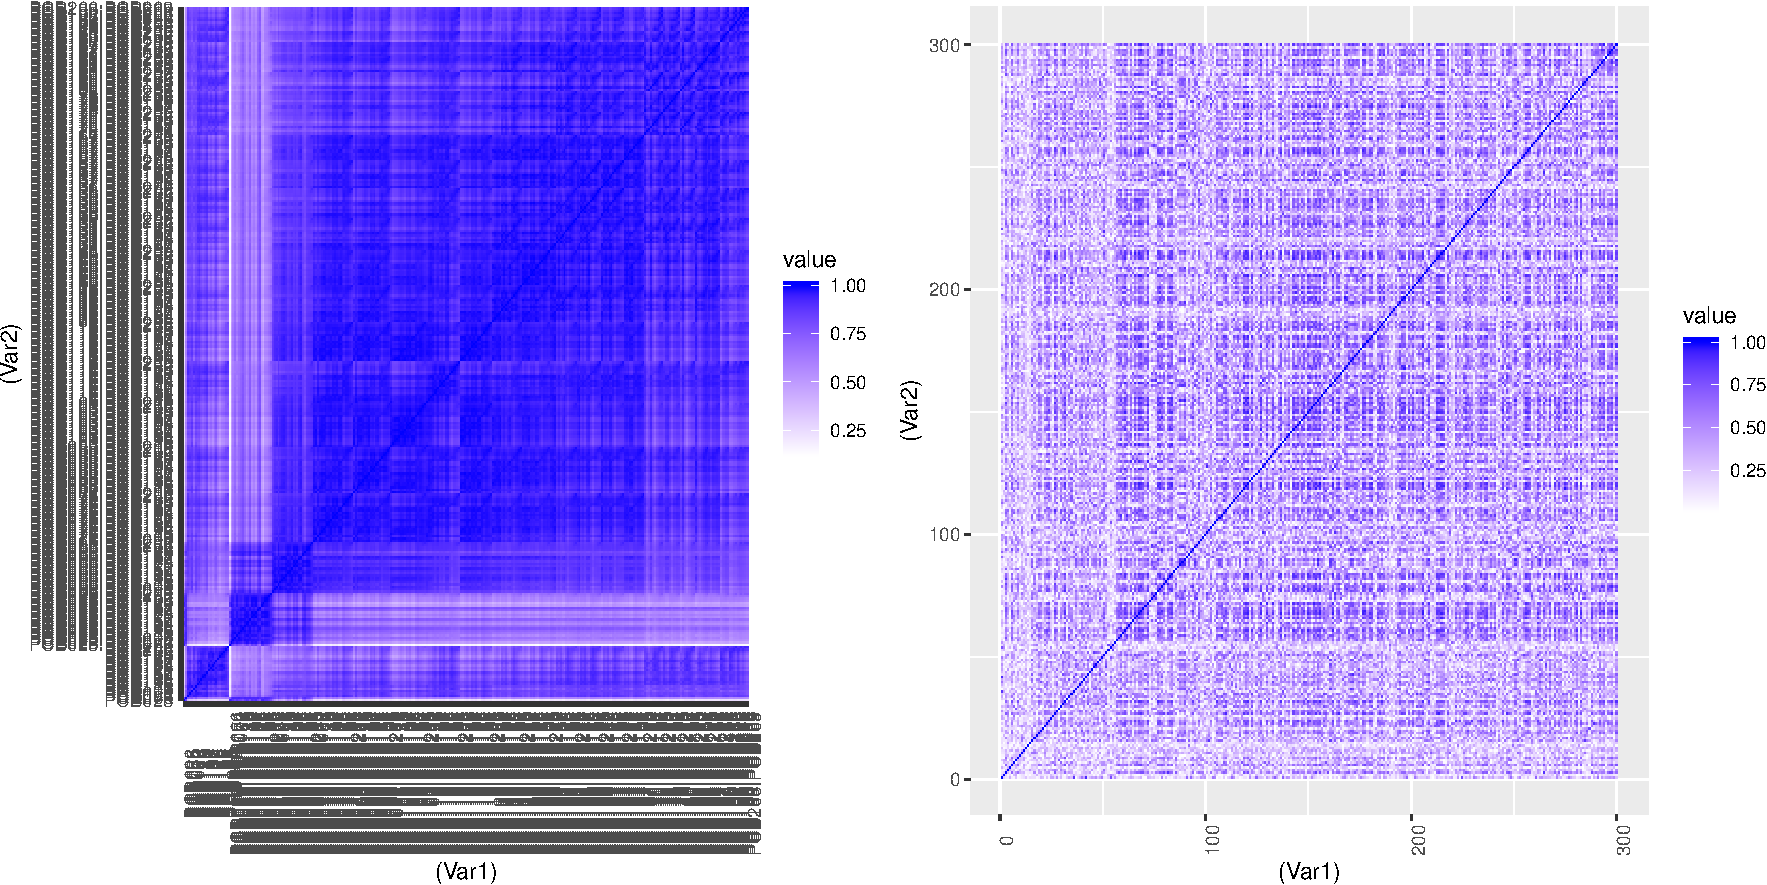
\includegraphics{Low_levels_covariance_files/figure-latex/unnamed-chunk-8-1.pdf}
\caption{Combined main and interaction 2005-2006}
\end{figure}

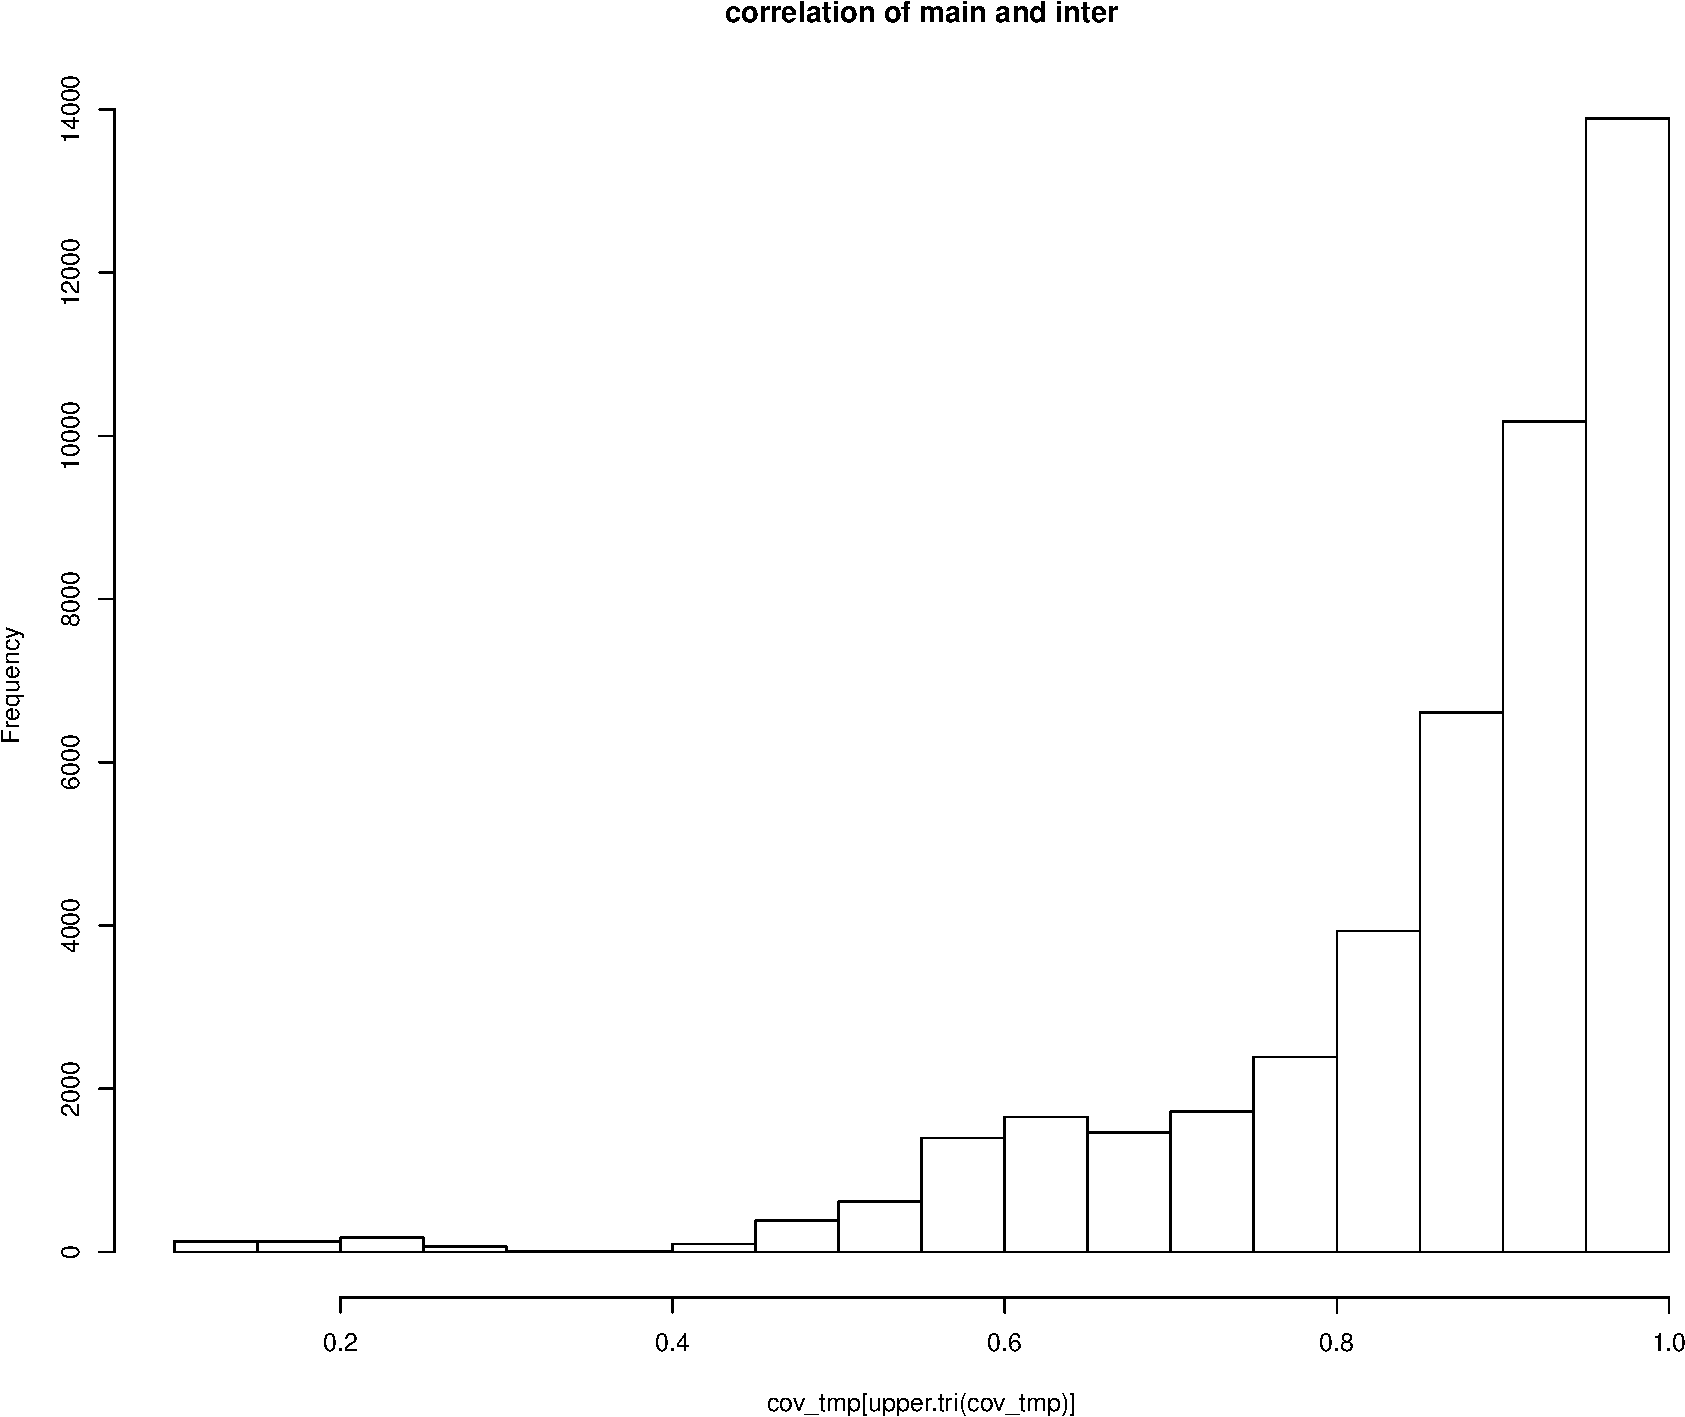
\includegraphics{Low_levels_covariance_files/figure-latex/unnamed-chunk-9-1.pdf}

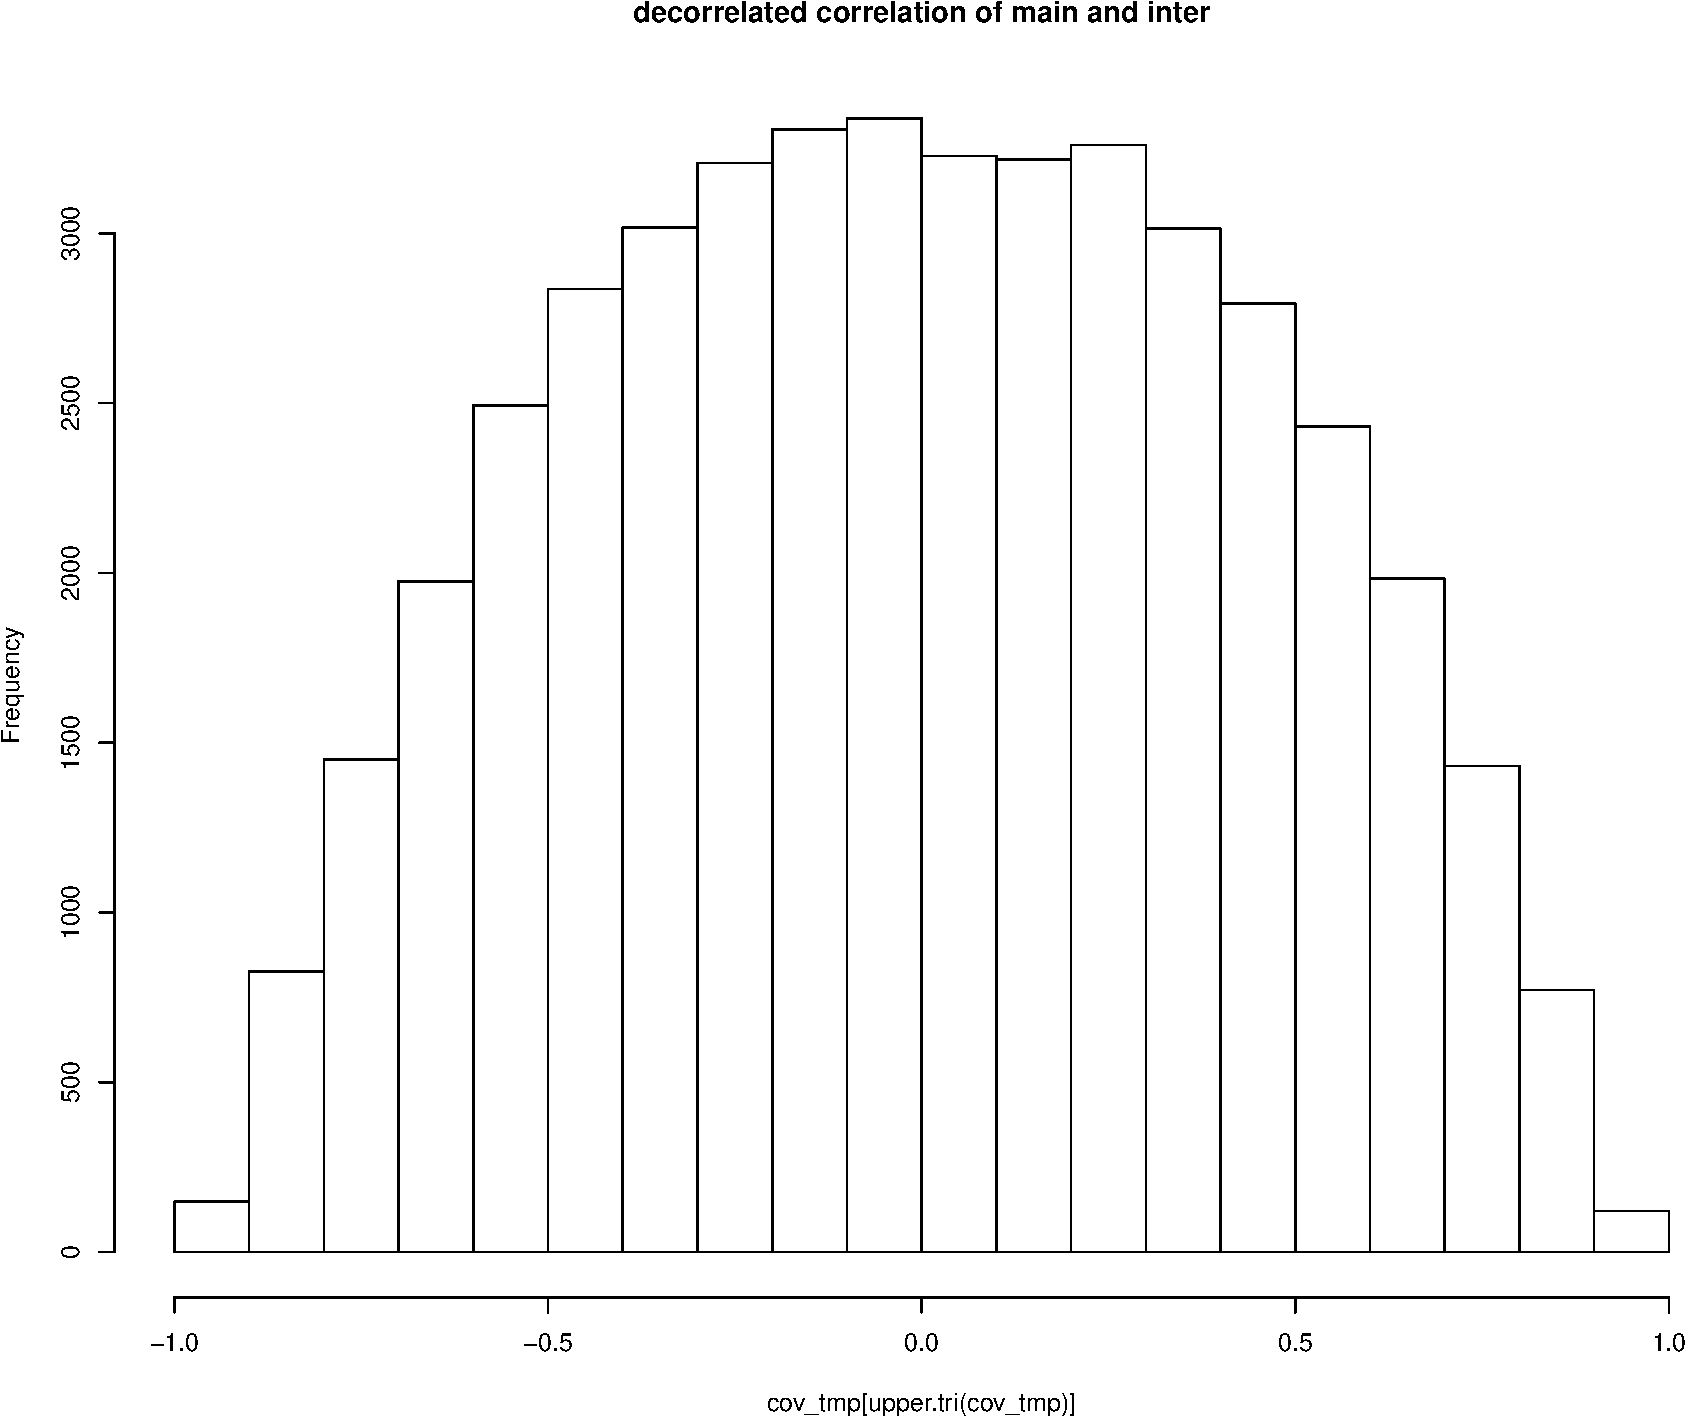
\includegraphics{Low_levels_covariance_files/figure-latex/unnamed-chunk-10-1.pdf}

\newpage

\subsection{Simulation setup}\label{simulation-setup}

\begin{enumerate}
\def\labelenumi{\arabic{enumi}.}
\tightlist
\item
  p = 231 for 1999 or 300 for 2005\\
\item
  \(n \in \{100, 150, p\}\)\\
\item
  the simulated covariates will follow Normal or Chi with df = 1\\
\item
  Variance estimation method will be GCTA and EigenPrism method\\
\item
  Iteration time is 100
\end{enumerate}

\section{Result}\label{result}

\subsection{1999}\label{section}

\begin{verbatim}
      n MSE est_var est_mean NA_total     method var_main_effect x_dist
 1: 100 626     138       32        9 EigenPrism              10    chi
 2: 150 790     140       36        0 EigenPrism              10    chi
 3: 231 740      61       36        0 EigenPrism              10    chi
 4: 100 852     242       35        0       GCTA              10    chi
 5: 150 848     191       36        0       GCTA              10    chi
 6: 231 702      66       35        0       GCTA              10    chi
 7: 100 504     100       30        4 EigenPrism              10 normal
 8: 150 604      74       33        0 EigenPrism              10 normal
 9: 231 700      70       35        0 EigenPrism              10 normal
10: 100 649     173       32        0       GCTA              10 normal
11: 150 656      99       34        0       GCTA              10 normal
12: 231 705     101       35        0       GCTA              10 normal
\end{verbatim}

\begin{verbatim}
      n  MSE est_var est_mean NA_total     method var_main_effect x_dist
 1: 100 16.9    16.9      9.7        0 EigenPrism              10    chi
 2: 150  9.4     9.5     10.0        0 EigenPrism              10    chi
 3: 231  5.2     5.2     10.2        0 EigenPrism              10    chi
 4: 100 19.0    18.5      9.1        0       GCTA              10    chi
 5: 150  8.5     8.6      9.9        0       GCTA              10    chi
 6: 231  4.8     4.9     10.1        0       GCTA              10    chi
 7: 100 19.2    19.4      9.9        0 EigenPrism              10 normal
 8: 150 13.3    13.2     10.5        0 EigenPrism              10 normal
 9: 231  4.6     4.6     10.0        0 EigenPrism              10 normal
10: 100 22.0    22.1      9.6        0       GCTA              10 normal
11: 150 13.0    13.0     10.3        0       GCTA              10 normal
12: 231  4.1     4.1     10.0        0       GCTA              10 normal
\end{verbatim}

\newpage

\subsection{2005}\label{section-1}

\begin{verbatim}
      n  MSE est_var est_mean NA_total     method var_main_effect x_dist
 1: 100  897     132       38        6 EigenPrism              10    chi
 2: 150 1131     140       41        0 EigenPrism              10    chi
 3: 300 1574     109       48       44 EigenPrism              10    chi
 4: 100 1274     287       41        0       GCTA              10    chi
 5: 150 1673     327       47        0       GCTA              10    chi
 6: 300 2090     213       53        0       GCTA              10    chi
 7: 100 1250     173       43        6 EigenPrism              10 normal
 8: 150 1162     129       42        0 EigenPrism              10 normal
 9: 300 1404     104       46       45 EigenPrism              10 normal
10: 100 1789     366       48        0       GCTA              10 normal
11: 150 1570     266       46        0       GCTA              10 normal
12: 300 2069     257       53        0       GCTA              10 normal
\end{verbatim}

\begin{verbatim}
      n  MSE est_var est_mean NA_total     method var_main_effect x_dist
 1: 100 16.4    15.8     10.9        0 EigenPrism              10    chi
 2: 150 13.3    11.6     11.3        0 EigenPrism              10    chi
 3: 300  4.5     4.6      9.9        0 EigenPrism              10    chi
 4: 100 12.3    11.2     11.1        0       GCTA              10    chi
 5: 150 11.0     7.7     11.8        0       GCTA              10    chi
 6: 300  3.7     3.0     10.9        0       GCTA              10    chi
 7: 100 15.1    13.6     11.3        0 EigenPrism              10 normal
 8: 150 11.4    10.6     11.0        0 EigenPrism              10 normal
 9: 300  6.7     6.7     10.3        0 EigenPrism              10 normal
10: 100 12.1    10.2     11.4        0       GCTA              10 normal
11: 150  9.4     7.2     11.5        0       GCTA              10 normal
12: 300  4.4     3.4     11.0        0       GCTA              10 normal
\end{verbatim}


\end{document}
